$\displaystyle \int_{1}^{3}\left(\frac{1}{2x-1}-\frac{1}{2x+1}\right)\,dx$

\nopagebreak
\begin{align*}
I &= \int_{1}^{3} \frac{dx}{2x-1} - \int_{1}^{3} \frac{dx}{2x+1} \\
&= \left[ \frac{1}{2} \ln|2x-1| \right]_{1}^{3} - \left[ \frac{1}{2} \ln|2x+1| \right]_{1}^{3} \\
&= \frac{1}{2} (\ln 5 - \ln 1) - \frac{1}{2} (\ln 7 - \ln 3) \\
&= \frac{1}{2} \ln 5 - \frac{1}{2} \ln \frac{7}{3} = \frac{1}{2} \ln \left( \frac{5}{7/3} \right) \\
&= \frac{1}{2} \ln \frac{15}{7}
\end{align*}

\[
\boxed{\displaystyle \frac{1}{2} \ln \frac{15}{7}}
\]

\begin{center}
    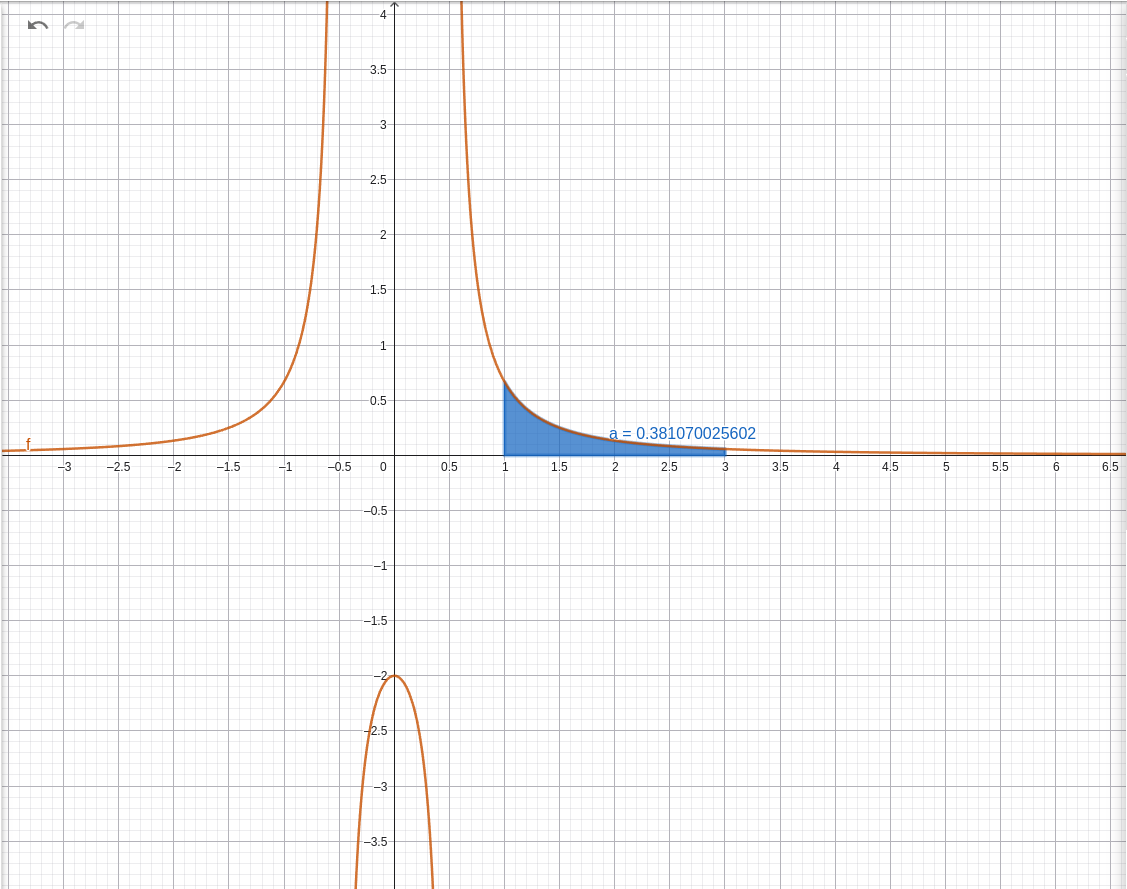
\includegraphics[width=0.5\textwidth]{Graficas/ejer12.png}
\end{center}
